\chapter{Binary Classifier}
\label{chap:classifier}

A practical application of the \gls{CLP} is the integration in the \gls{VRP}, where
a number of customers need to be served with a set of items by a fleet of vehicles that have
to start from a depot and return. The goal is to minimize the total distance driven
by the vehicles. When considering multidimensional items, the NP-hard problem itself,
increases in complexity, as every tour is representing a \gls{CLP} itself. \footcite[cf.][pp. 1--2]{tamke_branch-and-cut_2024}

The emphasis is placed primarily on \gls{ML}-based classifiers.
These are supervised \gls{ML} algorithms predicting the
value of a categorical or binary output column, called label, based on the
values of other columns, called features. Classifiers are supervised learning models,
which are trained on a labeled dataset,
where the correct output values are known in advance, and then use this knowledge to
make predictions on new, unseen data. The accuracy can be evaluated afterwards by comparing
the predicted labels with the actual labels. \footcite[cf.][]{kotsiantis_supervised_2007}
An exemplary train dataset is shown in Table~\ref{tab:classifier_label_data}.

\input{tables/label_classifier}

A classifier can be trained using various \gls{ML} models such as \gls{LR},
\gls{ANN}, support vector machines, or others. However, the most crucial aspect of any
\gls{ML} model is the selection of data, particularly the choice of features and
the size of the training set, since many models can be implemented from available
libraries and be compared performance wise. The model attempts to learn correlations between the provided features
and the corresponding labels. If the features are poorly chosen, the model may fail
to capture the underlying patterns in the data. Additionally, if the training set
is too small, the model might not generalize well, ultimately lacking the ability
to accurately predict unseen data. Furthermore, it needs to be noted, that available
\gls{ML} models are not by nature superior to other models, but can significantly outperform
other models on specific application problem \footcite[cf.][pp. 250, 264]{kotsiantis_supervised_2007}.


\section{Evaluation metrics for ML approaches}
\label{sec:classifier_objectives}
To compare different models and \gls{ML} approaches performance indicators are needed. The most common
measures rely on the binary output of the confusion matrix, which sorts the output along
their true and predicted labels. The predicted labels of the \gls{ML} model are
divided in two groups via a certain threshold, usually 0.5, with all predicted values above it,
considered in the predictive positive column and below it, in the predicted negative column.

\begin{table}[ht]
    \centering
    \begin{tabular}{@{}lcc@{}}
        \toprule
                                 & \textbf{Predicted Positive} & \textbf{Predicted Negative} \\
        \midrule
        \textbf{Actual Positive} & \Gls{TP}                    & \Gls{FN}                    \\
        \textbf{Actual Negative} & \Gls{FP}                    & \Gls{TN}                    \\
        \bottomrule
    \end{tabular}
    \caption{Confusion matrix (binary classification).}
    \label{tab:confusion_matrix}
\end{table}
The output can be used to calculate the accuracy and the F1-score of the classification, which
helps to interpret the outcomes and compare different model types:
\begin{align}
    \text{Accuracy}=\frac{TP+TN}{TP+FN+TN+FP}
    \qquad
    \text{F1}=\frac{2\,TP}{2\,TP+FP+FN}
\end{align}
The accuracy is the ratio between the true classified classes against the whole population
of predictions. The F1-score emphasis the \gls{TP} labels and is therefore especially
often used for classification purposes. Both metrics have the perfect score with 1, and the worst with 0.
However, these evaluation metrics draw too optimistic a picture of the model performance,
when the dataset is imbalanced, as one class is dominating the other. Imbalance is occurrent,
when the classes representing each label, feasible and infeasible, have a huge size difference.\footcite[cf.][p. 2f.]{chicco_advantages_2020}
Two alternatives are firstly the \gls{MCC}, which is robust against imbalance
and focuses on both prediction labels. \gls{MCC} has the advantage to account the majority of the predictions
relative to class size and is defined from -1 to 1. However, if one class of the confusion
matrix has a population size of 0 \gls{MCC} is not defined.\footcite[cf.][p.5]{chicco_advantages_2020}
\begin{align}
    \text{MCC}=\frac{TP*TN - FP*FN}{\sqrt{(TP+FP)*(TP+FN)*(TN+FP)*(TN+FN)}}
\end{align}
Secondly, the \gls{AUROC},where several thresholds are used
to calculate the \gls{TPR} and the \gls{FPR} for different acceptance steps,
which indicates how well the classification does in general terms. \footcite[cf.][p.2f.]{chicco_advantages_2020}
\begin{align}
    \text{TPR}=\frac{TP}{TP+FN}
    \qquad
    \text{FPR}=\frac{TN}{FP+TN}
\end{align}
The following Plot~\ref{fig:AUROC_curve} shows several receiver operating curves and their corresponding \gls{AUROC} values, also shown
in the legend. The baseline is the angle bisector indicating random guessing with an \gls{AUROC} value of 0.5. The bigger the area under the
curve gets, the better is the fit. The perfect fit is displayed, when the full square is covered under the receiver operating curve.

\begin{figure}[ht]
    \centering
    \begin{tikzpicture}
        \begin{axis}[
            axis lines=middle,
            axis line style = {-Stealth[{length=6pt}]},
            samples=200,
            domain=0:1,
            ymin=0, ymax=1,
            xtick={0,0.2,0.4,0.6,0.8,1},
            ytick={0,0.2,0.4,0.6,0.8,1},
            width=10cm,
            height=6cm,
            legend style={at={(1.05,0.5)},anchor=west},
            ylabel near ticks,
            xlabel near ticks,
            xlabel={$FPR$},
            ylabel={$TPR$},
            nodes near coords,
            every node near coord/.append style={anchor=north}, % shift label to right
            point meta=explicit symbolic
            ]
            % LCurves
            \addplot[name path = xaxis, forget plot] coordinates {(0,0) (1,0)};

            \addplot[green,thick, name path=a]coordinates {(0,0) (0,1) (1,1)};
            \addlegendentry{Perfect Fit (1)}

            \addplot[teal, thick, name path=b] {-(x-1)^8 + 1};
            \addlegendentry{Good Fit  (0.89)}

            \addplot[blue, thick, name path=c] {-(x-1)^2 + 1};
            \addlegendentry{Fit (0.67)}

            \addplot[black,thick,name path=d] {x};
            \addlegendentry{Random guessing (0.5)}

            %\legend{Perfect Fit (1), Good Fit  (0.89), Fit (0.67), Random guessing (0.5)}
            %\addplot [only marks, mark = o,mark size=2pt] coordinates {(0.05, 0.47) [A](0.11,0.99)    [B]};
            \addplot[fill=green, draw=none, opacity=0.1, forget plot] fill between [of=a and xaxis];
            \addplot[fill=teal, draw=none, opacity=0.1, forget plot] fill between [of=b and xaxis];
            \addplot[fill=blue, draw=none, opacity=0.1, forget plot] fill between [of=c and xaxis];
            \addplot[fill=black, draw=none, opacity=0.1, forget plot] fill between [of=d and xaxis];

            % Dotted lines for y=0 and y=1
            \addplot[gray,thick, forget plot] coordinates {(1,0) (1,1)};
        \end{axis}
    \end{tikzpicture}
    \caption[Example of possible AUROC values.]{Example of possible \gls{AUROC} values.}
    \label{fig:AUROC_curve}
\end{figure}

To highlight the differences between an imbalanced and balances training dataset, two classifications and their respective
evaluation metrics with exception of the \gls{AUROC} are compared.

\begin{table}[ht]
    \centering
    \begin{tabular}{@{}P{0.1\textwidth}P{0.38\textwidth}P{0.38\textwidth}@{}}
        \toprule
        Score  & Balanced Dataset A $(n = 100)$                                   & Imbalanced Dataset B  $(n = 100)$                            \\
        \midrule
        Bal.   & Pos = 50; Neg = 50                                               & Pos = 91; Neg = 9                                            \\
        \midrule
        Distr. & TP = 47; FN = 3; TN = 5; FP = 45                                 & TP = 90; FN = 1; TN = 1; FP = 8                              \\
        \midrule
        Acc    & $\frac{47 + 5}{47 + 3  + 5 + 45} = 0.52$                         & $\frac{90 + 1}{90 + 1  + 1 +8} = 0.91$                       \\
        \midrule
        F1     & $\frac{2* 47}{2*47 + 3 + 45} = 0.66$                             & $\frac{2 * 90}{2 * 90 + 1 +8} = 0.95$                        \\
        \midrule
        MCC    & $\frac{47*5 -3*45*1}{\sqrt{(47+45)*(47+3)*(5+45)*(3+5)}} = 0.07$ & $\frac{90*1 - 8*1}{\sqrt{(90+8)*(90+1)*(1+8)*(1+1)}} = 0.21$ \\
        \bottomrule
    \end{tabular}
    \caption[Comparison of Accuracy, F1-score and MCC with an exemplary balanced and unbalanced
        dataset.]{Comparison of Accuracy, F1-score and MCC with an exemplary balanced and unbalanced
        dataset.\footnote{Numbers and examples are inspired on \cite[p.9]{chicco_advantages_2020}}}
    \label{tab:indicator_comparison}
\end{table}
In these two examples weaknesses of classical evaluation metrics are apparent. In the first
example the positive and negative label classes are equal, and the distribution for the
labels is more or less random, as the sum of the false predicted values is almost equal to
the true predicted values. The accuracy and the \gls{MCC} indicate this random guessing
behavior with values close to the middle of the respective indicator range.
The accuracy is slightly positive as the rate of true predicted values of the positive class
with $94\%$ is very high. As the dataset is balanced classic metrics can still grasp
the poor performance of the classifier. However, when looking at the second example, both
accuracy and F1-score have very high values indicating very good performance, but this is
due to the imbalanced class distribution. In the negative class with 9 samples, only $11\%$
are correctly classified, this poor performance is shown with a low \gls{MCC} score. It needs
to be noted, that in every example it needs to be chosen, where the optimization focus should
be laid to, if only the \gls{TPR} is from interest F1-score serves well.\footcite[cf.][p.8f.]{chicco_advantages_2020}
The next section will dive deeper how the routes for the training data are retrieved.


\section{Data Retrieval}
\label{sec:DataRetrieval}
Collecting the training data is one crucial step, for the model creation and two approaches exist.

\subsubsection{Saving labeled routes from exact algorithms (Save strategy)}
The first one is to save all routes with exact loading label from an exisiting \gls{3L-CVRP}
algorithm, as \cite{zhang_learning-based_2022} did in their paper. However the binary classifier
was integrated used in the same exact algorithm
and therefore the solution structure of routes in the train data is similar to the real data afterwards. \footcite[cf.][]{zhang_learning-based_2022}
To follow this approach the exact branch-and-cut algorithm from \cite{tamke_branch-and-cut_2024} was
used to save all routes, which are labeled and found in an 8-hour timelimit from an instance. The routes
are saved based on their respective \gls{LoadSt} and \gls{LoadFl}. The \gls{LoadSt} sorts the routes in the
label categories feasible, infeasible, unknown and invalid and is determined by the exact \gls{CP} solver.
If the solver could not find a concrete Feasible/ Infeasible label in the timelimit fot the solver the route
will be classified as invalid or unknown, based on the resp. \gls{LoadFl}.
The \gls{LoadFl} defines the subset of
loading constraints used. Three \glspl{LoadFl} are considered in the orginal algorithm, which are shown
in the following:
\begin{itemize}
    \item All Constraints: $\mathcal{G}$
    \item No Support Area: $\mathcal{G}\setminus \{\text{SupportArea}\}$
    \item No Sequence: $\mathcal{G}\setminus \{\text{Sequence}\}$
\end{itemize}
During the algorithm labeled routes are saved based on these two categories. The concrete route sequence
is only relevant for the first two \glspl{LoadFl}, and the routes are saved as sequences. For the third
group \textit{No Sequence} the found routes are independent from their sequence and a respective set
of the customer ids without a order is saved. \footcites[Retrieved from][]{tamke_repository_2024}[cf.][]{tamke_branch-and-cut_2024}
After the branch-and-cut algorithme the routes are sorted into different sets composed of the \gls{LoadFl} and \gls{LoadSt}.
All the route sequences found are resepcted for the train dataset. However, as the permutation number of all combinations
of customer ids of the sets from the third \gls{LoadFl} \textit{No Sequence}, would dominate the train dataset number wise,
three random permutations are considered from each set. The following table highlights, which routes depending on the
\gls{LoadFl} and \gls{LoadSt} are considered for the final train dataset.

\begin{table}[ht]
    \centering
    \begin{tabular}{@{}
            P{0.20\textwidth} % AllConstraints
            P{0.20\textwidth} % NoSupport
            P{0.20\textwidth} % NoLIFO
            @{}}
        \toprule
        \textbf{All Constraints}     & \textbf{NoSupport}           & \textbf{NoLIFO}              \\
        \midrule
        \cellcolor{green!20}Feasible & Feasible                     & Feasible                     \\
        \cellcolor{red!20}Infeasible & \cellcolor{red!20}Infeasible & \cellcolor{red!20}Infeasible \\
        \cellcolor{red!20}Unknown    & \cellcolor{red!20}Unknown    & \cellcolor{red!20}Unknown    \\
        \bottomrule
    \end{tabular}
    \caption{Construction of training data from branch-and-cut routes. All green cells are labeled as feasible, and all
        red cells as infeasible data}
    \label{tab:train_data_BC_routes}
\end{table}

As the trained classifier is used in an algorithm considering all loading constraints, feasible tours
must fulfill all loading constraints, but infeasible tours from a subset of loading constraints
will also be infeasible, when more loading constraints are considered.\footcite[cf.][p.7]{tamke_branch-and-cut_2024} therefore
the distinction is made in Table~\ref{tab:train_data_BC_routes}.
As the same tour can occur in different infeasible / unknown sets
duplicated tours with the same label will be deleted before training the model. To distinguish this strategy, it will
be called \textit{Save Strategy}.

\subsubsection{Creating random routes (Random Strategy)}
An alternative to the first approach is to create random routes from the \gls{3L-CVRP} instances used.
These routes need to be labeled in feasible and infeasible routes regarding their loading.
A \gls{CLP} algorithm with high solution quality is needed to ensure the correct labels. As the heuristic approaches
presented in Section~\ref{sec:classical_solution_approaches} do not provide an optimal solution,
the best choice is to use an exact approach to determine, if all items fit into the container with the loading constraints.
For this purpose, the exact \gls{CP} model was extracted from \cite{tamke_repository_2024} to create
a standalone \gls{CP} solver, which can be called for just one route.\footcite[Stolen with permission from][]{tamke_repository_2024}
The random routes are created with the Algorithm~\ref{alg:rand_routes_generation}, and three parameters are introduced to
control the number of random routes found. As the pseudocode has a lot of details, the parameters and
functionalities are summarized in the following:

\begin{itemize}
    \item 4 Input Parameters
          \begin{itemize}
              \item Multiplier $\alpha$: Integer determining repetitions ($n\times\alpha$) for each route length $n$
              \item  Attempts limit $\beta$: Integer determining max failures per repetition
              \item  Success threshold $\gamma$: Integer determining success threshold per repetition
              \item Instance set $\mathcal{I}$: Set of instances routes should be generated from
          \end{itemize}
    \item Route length is starting with two customers increasing until no routes can be found
    \item Every new random route is checked, if the route is already contained in a route set
    \item Algorithm stops when no random route could be drawn in $n \times \alpha$ rounds
\end{itemize}

Generally the higher the parameters $\alpha$, $\beta$ and $\gamma$ are set and the more instances
are considered in the instance set $\mathcal{I}$, the more routes will be found. Different
random training datasets are presented in the Chapter~\ref{chap:computational_study}.
This strategy will be called \textit{Random Strategy}. In the nexr section three model candidates
are presented more in detail.

\section{Model Selection}
\label{sec:modelselection}
Every supervised learning method can predict the feasibility of a single loading, and the comparison
between different models is a tidious job. Therefore only three different classification
models will be explained in detail and compared in the computational study.
Two different types of models will be compared, regression and pure classification models. Regression
models are based on calculations and output a value between 0 and 1, which is then classified with
an artifical threshold in two distinct classes, as feasible and infeasible loading. Pure classification
models predict directly the label. \footcite[cf.][p.5]{nasteski_overview_2017}

\subsubsection{Logistic Regression}

The idea for \gls{LR} is based on linear regression, where either one or multiple independent explanatory
variables $\beta_i$ are multiplied with the feature values $X_i$ to sum up to a continuous scalar $\pi_i$.
The resulting model is the linear equation of the y-axis interception $\beta_0$
and the gradient variables $\beta_i$.
These explanatory variables are fitted to the population of samples by minimizing the mean squared
error. Afterwards the model can be used to predict new data points.\footcite[cf.][pp. 6-7]{nasteski_overview_2017}
The linear regression formula is depicted in the following, indicating the usage of vectors with bold font.
\begin{align}
    \pi_i=\beta_0+\beta_0*X_i+\dots+\beta_n*X_n = \beta_0 + \bm{\beta} * \bm{X}
    \label{eq:base_lr}
\end{align}
Linear regression is a very simple modeling approach and serves as a benchmark for many problems. As the Formula~\ref{eq:base_lr} is able to predict continuous
values, it is not possible to classify binary values. Therefore the output variable $\pi_i$ is transformed via a logistic function, called sigmoid function,
to model a continuous probability distribution with the formula:
\begin{align}
    \sigma(z)=\frac{1}{1+\exp^{-z}},\, \text{with } z = \beta_0 + \bm{\beta} * \bm{X}
    \label{eq:logistic_func}
\end{align}
The resulting logistic function is bound to the range of 0 and 1, and results can be interpreted
in two labels using an threshold. An output of 0.5 can be interpreted as random
guessing between both labels, as $z=0$. The curve of the logistic function is shown in Figure~\ref{fig:LR_plot}.
The model is fitted to predict feasible and infeasible loadings best.\footcite[cf.][]{kirasich_random_2018}
\begin{figure}[ht]
    \centering
    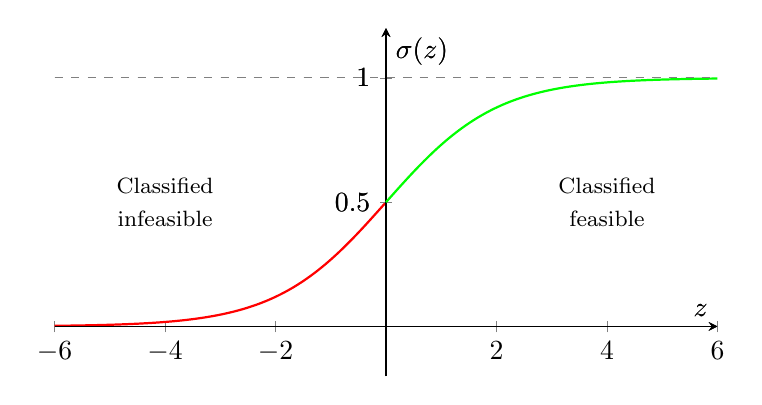
\begin{tikzpicture}
        \begin{axis}[
                axis lines=middle,
                xlabel={$z$},
                ylabel={$\sigma(z)$},
                samples=200,
                domain=-6:0,
                ymin=-0.2, ymax=1.2,
                xtick={-6,-4,-2,0},
                ytick={0,0.5,1},
                width=10cm,
                height=6cm,
            ]
            % Logistic function
            \addplot[red, thick] {1/(1+exp(-x))};

            %Text
            \node[rectangle,minimum width=24pt,align=center] (test)  at (-4,  0.5) {\footnotesize Classified \\ \footnotesize infeasible};

            % Dotted lines for y=0 and y=1
            \addplot[dashed, gray] coordinates {(-6,1) (6,1)};
        \end{axis}
        \begin{axis}[
                axis lines=middle,
                xlabel={$z$},
                ylabel={$\sigma(z)$},
                samples=200,
                domain=0:6,
                ymin=-0.2, ymax=1.2,
                xtick={2,4,6},
                ytick={0,0.5,1},
                width=10cm,
                height=6cm,
            ]
            % Logistic function
            \addplot[green, thick] {1/(1+exp(-x))};

            %Text
            \node[rectangle,minimum width=24pt,align=center] (test)  at (4,  0.5) {\footnotesize Classified \\ \footnotesize feasible};

            % Dotted lines for y=0 and y=1
            \addplot[dashed, gray] coordinates {(-6,1) (6,1)};
        \end{axis}
    \end{tikzpicture}
    \caption{Transformation of linear regression to logistic regression via the sigmoid function.}
    \label{fig:LR_plot}
\end{figure}



\subsubsection{Decision Trees}
Decision trees classify samples by sorting them based on their features. Every decision tree
is built up by three elements, one root node and several branches and leaves. The root node
depicts the starting point of the classification and is a branch, classifying the sample
regarding to one feature. At every level of the tree several branches are added, which can be followed
by either branches or leafes. Each branch splits the instance space into two or more sub-spaces
according to a certain threshold of the input values. A leaf is the exit point declaring
the label of the sample data.\footcite[cf.][p.5-6]{nasteski_overview_2017}
The following small decision tree (see Fig.~\ref{fig:decision_tree}) is an example,
how the loading could be classified with numerical features.

\begin{figure}[ht]
    \centering
    \begin{tikzpicture}[
            >=Latex,
            node distance=15mm and 0mm,
            decision/.style={rectangle, rounded corners=2pt, draw, fill=blue!8, align=center, inner sep=3pt},
            leafgood/.style={rectangle, rounded corners=2pt, draw, fill=green!10, align=center, inner sep=3pt},
            leafbad/.style={rectangle, rounded corners=2pt, draw, fill=red!10, align=center, inner sep=3pt},
            edge/.style={-Latex, thick}
        ]
        % Nodes
        \node[decision] (root) {Relative volume\\$> 70\%$?};

        \node[decision, below right=of root] (items) {Item count\\$> 30$?};
        \node[decision, below left=of root] (weight){Relative weight\\$> 80\%$?};

        \node[leafgood, below=of items, xshift=-14mm] (itemNo)  {Feasible};
        \node[leafbad, below=of items, xshift= 14mm] (itemYes) {Infeasible};

        \node[leafbad,  below=of weight, xshift=14mm] (wYes)   {Infeasible};
        \node[leafgood, below=of weight, xshift=-14mm] (wNo)    {Feasible};

        % Edges with labels
        \draw[edge] (root) -- node[above, sloped]{Yes} (items);
        \draw[edge] (root) -- node[above, sloped]{No}  (weight);

        \draw[edge] (items) -- node[left]{No}  (itemNo);
        \draw[edge] (items) -- node[right]{Yes} (itemYes);

        \draw[edge] (weight) -- node[right]{Yes} (wYes);
        \draw[edge] (weight) -- node[left]{No}  (wNo);

    \end{tikzpicture}
    \caption{Exemplary decision tree to understand classification.}
    \label{fig:decision_tree}
\end{figure}

The  prominent advantage is, that the logic behind the classification can be understood
completely. In this example all routes, with more than 30 items and $70\%$ volume utilization are classified infeasible,
as well as those tours where the relative weight utilization is above $80\%$, but the volume utilization is lower. The complex
$NP$-hard problem is to find the optimal binary decision tree and finding the optimal subset and order of
features.
When many levels of branches are added, and the decision tree grows in depth, the chance of
overfitting the decision tree to the training data is more likely. Therefore several control mechanisms
were developed to avoid this. The first one is to control the maximum depth (\textit{max\_depth})
of the decision tree. Secondly, after the decision tree is created, to prune it by removing leaves from
the tree and comparing it with an identical descision tree, if this has lowered the overall performance
and the third method is stopping the fitting algorithm before the data is perfectly fitted to. \footcite[cf.][p.252]{kotsiantis_supervised_2007}
One further advantage of decision trees is that the data does not need to to be scaled as every feature is
tested on feature own thresholds, in comparion of the other presented models.

\subsubsection{Feed Forward Neural Networks}

Neural networks are a collection of single perceptrons/ neuron, which are all internally connected and
,in the case of feed forward networks, signals are only allowed to go straight from input to output. One neuron
in the network is either defined as input, output or as hidden unit. One neuron calculates its
output similar to the \gls{LR} with $X_i$ feature values and $w_i$ weights, the output is defined
as $\sum_{i \in \mathcal{n}} X_i * w_i$ and can be truncated by a threshold forcing all about above 1
to be 1 and all negative values to be zero. Every unit signals its output calculated by an individual
activation function to all the next units of the next layer of the network. All the signals are
then interpreted at the output layer. For binary classification tasks the presented sigmoid function from \gls{LR} is used.
An exemplary neural network is shown in Figure~\ref{fig:ffnn}.\footcite[cf.][p.255]{kotsiantis_supervised_2007}

\begin{figure}[ht]
    \centering
    \begin{tikzpicture}[
            >=Latex,
            neuron/.style={circle, draw, minimum size=16pt, inner sep=0pt},
            input/.style={neuron, fill=blue!8},
            hidden/.style={neuron, fill=green!8},
            output/.style={draw, rounded corners=3pt, minimum width=24pt, minimum height=16pt, inner sep=2pt, fill=red!8},
            dotnode/.style={draw=none, fill=none, minimum size=6pt, inner sep=0pt},
            conn/.style={-Latex, thick},
            hiddenneuron/.style={circle, minimum size=16pt, inner sep=0pt},
        ]

        % Column x-positions
        \def\xin{0}
        \def\xhA{2.6}
        \def\xhB{5.2}
        \def\xout{7.8}
        \def\xcls{10.2}

        % ------- Inputs (show only x1, x2, ... , xn) -------
        \node[input] (x1)  at (\xin,  -1.2) {$x_1$};
        \node[input] (x2)  at (\xin,  -2.2) {$x_2$};
        \node[dotnode] (dots) at (\xin, -3.0) {$\vdots$};
        \node[input] (xn)  at (\xin,  -3.8) {$x_n$};

        %\node[above=6pt of x1] (inlab) {\small Inputs (features)};

        % ------- Hidden layer 1 (3 neurons) -------
        \node[hidden] (h1) at (\xhA, -1.2) {};
        \node[hidden] (h2) at (\xhA, -2.5) {};
        \node[hidden] (h3) at (\xhA, -3.8) {};
        %\node[above=6pt of h1] {\small Hidden layer 1};

        % ------- Hidden layer 2 (3 neurons) -------
        \node[hidden] (g1) at (\xhB, -1.2) {};
        \node[hidden] (g2) at (\xhB, -2.5) {};
        \node[hidden] (g3) at (\xhB, -3.8) {};
        %\node[above=6pt of g1] {\small Hidden layer 2};

        % ------- Output (sigmoid) -------
        \node[output, label=:{Sigmoid}] (y) at (\xout, -2.5) {$\hat{y}=s(z)$};
        \node[hiddenneuron] (_y) at (\xout - 0.55, -2.5) {};
        %\node[above=6pt of y] {\small Sigmoid output};

        % ------- Class labels (annotation) -------
        \node[output] (th) at (\xcls, -2.5) {\small thresh $0.5$};
        \node[neuron, minimum size=14pt] (y1) at (\xcls + 1.8, -1.6) {\small 1};
        \node[neuron, minimum size=14pt] (y0) at (\xcls + 1.8, -3.4) {\small 0};
        %\node[right=4pt of y1] {\small class if $\hat p>0.5$};
        %\node[right=4pt of y0] {\small else};

        % ------- Connections -------
        % Inputs -> Hidden1 (skip the dots node)
        \foreach \src in {x1,x2,xn} {
                \foreach \dst in {h1,h2,h3} {
                        \draw[conn] (\src) -- (\dst);
                    }
            }

        % Hidden1 -> Hidden2
        \foreach \src in {h1,h2,h3} {
                \foreach \dst in {g1,g2,g3} {
                        \draw[conn] (\src) -- (\dst);
                    }
            }

        % Hidden2 -> Output
        \foreach \src in {g1,g2,g3} {
                \draw[conn,shorten >=3pt] (\src) -- (_y);
            }

        % Output -> threshold -> class nodes (annotation)
        \draw[conn] (y) -- (th);
        \draw[conn] (th.north east) to[out=60,in=180] (y1.west);
        \draw[conn] (th.south east) to[out=-60,in=180] (y0.west);

    \end{tikzpicture}
    \caption[An exemplary feed forward neural network with sigmoid output function.]{An exemplary feed forward neural network with sigmoid output function. Blue nodes are input, green ones hidden and red nodes output nodes.}
    \label{fig:ffnn}
\end{figure}

The training of the single layers and deciding which layers should be used is a complex task
and modern libraries as PyTorch are supporting with prebuilt models and analysis functions to choose
a good setup. Generally a \gls{FFNN} can be considered as an advanced \gls{LR} model,
which allows also nonlinear functions to be used for the processing of signals.

\parbreak
\cite{kotsiantis_supervised_2007} states, that no supervised \gls{ML} method is superior to another,
but each has its own advantages and disadavantages, which need to be considered.
Therefore all three different types are included in this work to compare performances, and
to understand the complexity of the underlying classification problem. As \gls{FFNN} normally
tend to need a large sample size and perform good with continuous data and  decision trees can be
trained on much smaller samples and perform good with mixed datatypes consisting of discrete/binary
and continuous values.\footcite[cf.][pp. 262ff.]{kotsiantis_supervised_2007}
\gls{LR} is a standard method and the easiest to implement and to train, and can dominate
other approaches due to their simplicity and interoperability. \footcite[cf.][p.8]{kirasich_random_2018}
In the following section the features used for training the single models are presented.
In Chapter~\ref{chap:computational_study} the performance of the single models is compared.

\begin{comment}
\section{Model Training}
\label{sec:ModelTraining}

Training is based on which model selected, XGBoost or /gls{FFNN} from pytorch library or others. Afterwards the Mini batch descent
algorithm to train the model!
\end{comment}

\section{Features}
\label{sec:Features}

Features are the most important puzzle piece for training a \gls{ML} model, as they portray the reality in numerical values, trying to
reduce the complexity without the loss of meaningfulness. In the presented case the loading feasibility probability of single tours.
The complete feature list spans 48 features, which can be divided in three groups to understand the underlying logic.

\begin{itemize}
    \item 2 General Features: General information about each tour
    \item 10 Loading Constraint Features: Concepted to depict the loading constraint set $\mathcal{G}$
    \item 36 Geometrical Ratio Features: Contain several geometrical ratio of items and container size to retrieve
          statistical values of minimum, maximimum, mean and standard deviation
\end{itemize}

Some additional definitions to Section~\ref{sec:mathematical_formulation}
are necessary to define the features formally. Following the mathematical definition, every route consists of the customers
from the subset $S \subseteq C$. Items of the set of item types $M$ is requested in different quantities by all customers $C$.
Each item type $m_j$ has its own dimensions height $z_j$, length $x_j$, width $y_j$, weight $q_j$ and fragility flag $f_j$.
The loading flag contains binary values of either 0 (nonfragile) or 1 (fragile).
Each customer $i$ demands $d_{ij}$ units of item type $j$.
The total weight, volume and quantity requested by a customer $i$ or the whole subset $S$ is calculated then by:

\[q(i) = \sum_{j \in M} q_j * d_{ij}\;\text{, resp. } q(S) = \sum_{i\in S} q(i)\]
\[v(i) = \sum_{j \in M} v_j * d_{ij}\;\text{, resp. } v(S) = \sum_{i\in S} v(i)\]
\[d(i) = \sum_{j \in M} d_{ij}\;\text{, resp. } D(S) = \sum_{i\in S} d(i)\]

Furthermore it is necessary to define the homogeneous fleet of vehicles
further. Every vehicle $k$ has the same dimensions of height $z_k$, length $x_k$ and width $y_k$ resulting in the maximum volume limit per
vehicle $Q = x_k *y_k*z_k$. As all vehicles are identical, the indices are obsolent, but are kept to distinguish clearer
from the item properties.

\subsubsection{General Features}
These two feature contain the number of customers $|S|$ in the respective route without the depot, and the total number of items requested by
this subset of customers $D(S)$.

\subsubsection{Loading Constraint Features}

The constraints are given in the Table~\ref{tab:loading_constraints_features} with the formula calculating the feature as well as the set of
loading constraints this feature is belonging to. The distinction, which loading constraints are described by which feature, is not
unambiguously, as several features can be adressed. The range of values is given in the last column with $h$ representing any number in $\mathbb{N}^{+}$.
All of the features presented have only values relative to the instance specific dimensions and weight limit of the vehicle, as these values
differ between different datasets, but also within the \gendreauDataSetText dataset. \footcite[cf.][p. 346]{gendreau_tabu_2006}
Capuring the \gls{LIFO} constraint is the most challenging task as multidimensionality and order is complex to be describe numerically
with one value. Therefore certain customer specific values, as relative volume/ weight or the share of fragile items, is multiplied
with the order in which the customers are driven to. \textit{Fragile Sequence} depicts the difficulty to load fragile items
in the beginning as further items need to be likely placed upon the first items.

\begin{table}[ht]
    \centering
    \renewcommand{\arraystretch}{2.0}
    \begin{tabular}{@{}P{0.08\textwidth}P{0.16\textwidth}P{0.26\textwidth}P{0.28\textwidth}@{}P{0.1\textwidth}@{}}
        \toprule
        No & Name                                                                                            & Constraint(s)          & Calculation                                                                                       & Range   \\
        \midrule
        1  & Relative Volume                                                                                 & Loading Capacity       & $\displaystyle\frac{v(S)}{V}$                                                                     & [0,1]   \\
        2  & Relative Weight                                                                                 & Loading Capacity       & $\displaystyle\frac{q(S)}{Q}$                                                                     & [0,1]   \\
        3  & Total Relative Length Items\footcite[Feature is adapted from][p.21]{sarah_de_wolf_machine_2022} & Stability, Orientation & $\displaystyle\frac{1}{x_k} * \sum_{i \in S}\sum_{j \in M} d_{ij} * x_j$                          & [0,$h$] \\
        4  & Total Relative Width Items \footnotemark[\value{footnote}]                                      & Stability, Orientation & $\displaystyle\frac{1}{y_k} * \sum_{i \in S}\sum_{j \in M} d_{ij} * y_j$                          & [0,$h$] \\
        5  & Total Relative Height Items  \footnotemark[\value{footnote}]                                    & Stability, Capacity    & $\displaystyle\frac{1}{z_k} * \sum_{i \in S}\sum_{j \in M} d_{ij} * z_j$                          & [0,$h$] \\
        6  & Ratio Fragile Items                                                                             & Fragility              & $\displaystyle\frac{1}{D(S)} * \sum_{i \in S}\sum_{j \in M} d_{ij} * f_j$                         & [0,1]   \\
        7  & Fragile Sequence                                                                                & Fragility, \gls{LIFO}  & $\displaystyle\sum_{i \in S}p_i * \frac{1}{d(i)}\sum_{j\in M} d_{ij}*f_j $                        & [0,$h$] \\
        8  & Volume Balance                                                                                  & Capacity, \gls{LIFO}   & $\frac{\displaystyle\sum\nolimits_{i \in S}p_i * v(i)}{\displaystyle\sum\nolimits_{i \in S}v(i)}$ & [0,$h$] \\
        9  & Volume Distribution                                                                             & Capacity, \gls{LIFO}   & $\displaystyle\frac{1}{V}*\sum_{i \in S}p_i * v(i)$                                               & [0,$h$] \\
        10 & Weight Distribution                                                                             & Capacity, \gls{LIFO}   & $\displaystyle\frac{1}{Q}\sum_{i \in S}p_i * q(i)$                                                & [0,$h$] \\
        \bottomrule
    \end{tabular}
    \caption{Loading constraints related features}
    \label{tab:loading_constraints_features}
\end{table}

\clearpage

\subsubsection{Geometrical Ratio Features}
The third and last feature group
was partly used by \cite{zhang_learning-based_2022} and is expanded for additional geometrical ratios applicable to three-dimensional loading.\footcite[cf.][p. 14]{zhang_learning-based_2022}
All geometrical ratios express the relation between two geometrical properties of either one item or one item to the vehicle. These ratios
are calculated for each item demanded from $S$ and afterwards the minimum, maximum, meand and standard deviation is calculated
from the $D(S)$ ratios, which are used as features. These ratios are expressed visually in the following Figure~\ref{fig:geometrical_ratio_features}.


\begin{figure}[ht]
    \centering

    % ---- Row 1: ratios between item dims & against container (L/H, W/H, W/L, L/CL, H/CH) ----
    \PanelItemDimDim{Width Height \\ \footnotesize{[0,$h$]}}{3}{2}
    \PanelItemDimDim{Length Height\\ \footnotesize{[0,$h$]}}{1}{2}
    \PanelItemDimDim{Width Length\footcite[Featues adapted from][p.14]{zhang_learning-based_2022}\\ \footnotesize{[0,$h$]}}{2}{3}
    \vspace{25pt}
    \PanelHeightOverArea{Height Area\\ \footnotesize{[0,1]}}
    \vspace{25pt}
    \PanelItemVsCont{Length Container Length\footnotemark[\value{footnote}]\\ \footnotesize{[0,1]}}{1}
    \PanelItemVsCont{Height Container Height\footnotemark[\value{footnote}]\\ \footnotesize{[0,1]}}{2}
    \PanelItemVsCont{Width Container Width\\ \footnotesize{[0,1]}}{3}
    \PanelAreaOverContArea{ItemArea ContainerArea\footnotemark[\value{footnote}]\\ \footnotesize{[0,1]}}
    \PanelVolumeOverContVolume{ItemVolume ContainerVolume\\ \footnotesize{[0,1]}}
    \caption[Nine geometric ratio feature icons.]{Nine geometric ratio feature icons. In each panel, the \textcolor{numC}{numerator is green}
        and the \textcolor{denC}{denominator is red}.
        \label{fig:geometrical_ratio_features}}
\end{figure}

All these nine geometrical features grasp the geometrical description of all items and is further outlined in the following example:
When we consider a route, where these three items are requested, described by their geometrical dimensions \{height, length, width\}:
\[
    \mathcal{I} = \{(12,5,10),\,(10,3,6),\,(10,10,10)\}
\]

\[
    \text{Width--Length Ratios: }
    \frac{y_j}{x_j} = \{2,\,2,\,1\}
\]

\[
    \begin{array}{c|c|c|c}
        \text{Min} & \text{Max} & \text{Mean} & \text{Std. Dev.} \\
        \hline
        1          & 2          & 1.67        & 0.471            \\
    \end{array}
\]

For every geometrical ratio the four features are calculated with this approach and are added to the model.

\parbreak

As the number of 48 features is huge for describing a rather simple problem in comparison to picture detection, the next steps
involve the analysis, which features have the greatest impact and which features can be dropped due to high correlation to other
features or to irrelevance to the prediction accuracy of the binary classifier.

\section{Feature Selection}
\label{sec:feature_engineering}

The selection of a subset of features helps to simplify the model
while preserving the same performance. For this procedure several frameworks have been published. In this work
the \gls{FSFS} is used. The procedure starts with a minimum number of features to start with, which are
preselected based on the best performance of the whole set of features. Iteratively in the \gls{FSFS} a new
feature is added to the model and it is tested, if the current fit of the model features need to be adapted.
This process is either repeated until no more features can be selected or a chosen bound for the maximum
feature number is reached. The theoretical background for the feature selection is, that the performance
of the model is optimal with the full feature set due to the noise and correlation between the features,
but somewhere in the middle. The following Figure~\ref{fig:feature-performance} shows this ideal feature-performance curve.

\begin{figure}[ht]
    \centering
    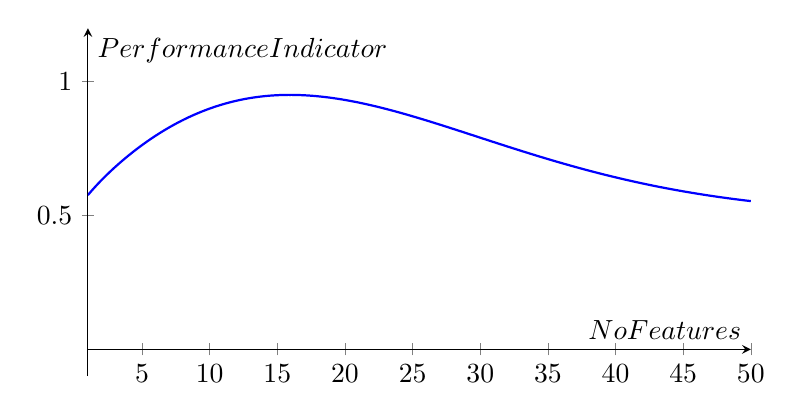
\begin{tikzpicture}
        \begin{axis}[
                axis lines=middle,
                xlabel={$No Features$},
                ylabel={$Performance Indicator$},
                samples=1000,
                domain=1:50,
                xmin=1, xmax=50,
                ymin=-0.1, ymax=1.2,
                xtick={5,10,15,20,25,30,35,40,45,50},
                ytick={0,0.5,1},
                width=10cm,
                height=6cm,
            ]
            \pgfmathsetmacro{\kap}{1.8}
            \pgfmathsetmacro{\lam}{0.04}

            \addplot[blue, thick] { 0.5 + 14*( \lam*\kap*(\lam*x)^(\kap-1)*exp( -(\lam*x)^\kap ) ) };


        \end{axis}
    \end{tikzpicture}
    \caption{Ideal curve of model performance determined by number of features selected.}
    \label{fig:feature-performance}
\end{figure}

The performance, e.g. the \gls{MCC} score, increases slowly until a maximum and then decresases slowly with
increasing number of features respected. The real curve observed will be not this extreme as the core
classfication system is always part, but should illustrate the benefits of feature selection.

When only one dataset is available, then the feature selection is a quite simple process, however, when
several datasets are available with different samples and retrieval methods it is very likely,
that with every feature selection a different subsets of features is selected. Therefore the
following procedure will be conducted:
\begin{algorithm}[htb]
    \caption{Feature and Dataset Selection}\label{alg:feature_dataset_selection}
    \begin{algorithmic}[1]
        \Procedure{Feature Dataset Selection}{Set of datasets $\mathcal{D}$}
        \For{$d \in D$}
        \State{Apply \gls{FSFS} to $d$ and determine optimal feature list $d_f$}
        \State{Save model $d_m$ with feature list $d_f$}
        \For{$d' \in D\setminus\{d\}$}
        \State Label dataset $d'$ with model $d_m$ and features $d_f$
        \State Calculate accuracy, F1-score, \gls{MCC} and \gls{AUROC}
        \State Save results
        \EndFor
        \EndFor
        \State{\textbf{return} Dataset $d$ with best performance over all datasets}
        \EndProcedure
    \end{algorithmic}
\end{algorithm}

To select the best fitting dataset and corresponding feature list for every dataset is iteratively
the optimal feature list selected with \gls{FSFS} and afterwards all other datasets are labeled
with the pretrained model and the selected features. This procedure is repeated for every dataset
and the dataset and the corresponding model and feature list is chosen, which has the best overall
performance. The performance is compared in this order: \gls{MCC}, \gls{AUROC}, F1-score and accuracy.
